% The comment below tells Rubber to compile the .dot files.
%
% rubber: module graphics
% rubber: rules rules.ini

\documentclass{beamer}

\usetheme{default}

\usefonttheme{structurebold}
\usepackage{helvet}
\usecolortheme{seagull}         % white on black

\usepackage[utf8]{inputenc}
\PassOptionsToPackage{hyphens}{url}\usepackage{hyperref,xspace,multicol}
\usepackage[absolute,overlay]{textpos}
\usepackage{tikz}
\usetikzlibrary{arrows,shapes,trees,shadows,positioning}
\usepackage{fancyvrb}           % for \Verb

% Remember the position of every picture.
\tikzstyle{every picture}+=[remember picture]

\tikzset{onslide/.code args={<#1>#2}{%
  \only<#1>{\pgfkeysalso{#2}} % \pgfkeysalso doesn't change the path
}}

% Colors.
\definecolor{guixred1}{RGB}{226,0,38}  % red P
\definecolor{guixorange1}{RGB}{243,154,38}  % guixorange P
\definecolor{guixyellow}{RGB}{254,205,27}  % guixyellow P
\definecolor{guixred2}{RGB}{230,68,57}  % red S
\definecolor{guixred3}{RGB}{115,34,27}  % dark red
\definecolor{guixorange2}{RGB}{236,117,40}  % guixorange S
\definecolor{guixtaupe}{RGB}{134,113,127} % guixtaupe S
\definecolor{guixgrey}{RGB}{91,94,111} % guixgrey S
\definecolor{guixdarkgrey}{RGB}{46,47,55} % guixdarkgrey S
\definecolor{guixblue1}{RGB}{38,109,131} % guixblue S
\definecolor{guixblue2}{RGB}{10,50,80} % guixblue S
\definecolor{guixgreen1}{RGB}{133,146,66} % guixgreen S
\definecolor{guixgreen2}{RGB}{157,193,7} % guixgreen S

\setbeamerfont{title}{size=\huge}
\setbeamerfont{frametitle}{size=\huge}
\setbeamerfont{normal text}{size=\Large}

% White-on-black color theme.
\setbeamercolor{structure}{fg=guixorange1,bg=black}
\setbeamercolor{title}{fg=white,bg=black}
\setbeamercolor{date}{fg=guixorange1,bg=black}
\setbeamercolor{frametitle}{fg=white,bg=black}
\setbeamercolor{titlelike}{fg=white,bg=black}
\setbeamercolor{normal text}{fg=white,bg=black}
\setbeamercolor{alerted text}{fg=guixyellow,bg=black}
\setbeamercolor{section in toc}{fg=white,bg=black}
\setbeamercolor{section in toc shaded}{fg=white,bg=black}
\setbeamercolor{subsection in toc}{fg=guixorange1,bg=black}
\setbeamercolor{subsection in toc shaded}{fg=white,bg=black}
\setbeamercolor{subsubsection in toc}{fg=guixorange1,bg=black}
\setbeamercolor{subsubsection in toc shaded}{fg=white,bg=black}
\setbeamercolor{frametitle in toc}{fg=white,bg=black}
\setbeamercolor{local structure}{fg=guixorange1,bg=black}

\newcommand{\highlight}[1]{\alert{\textbf{#1}}}

\title{Your distro is a Scheme library}
\subtitle{Hacking your way through the GNU~Guix API}

\author{Ludovic Courtès}
\date{\small{FOSDEM 2016}}

\setbeamertemplate{navigation symbols}{} % remove the navigation bar

\begin{document}

\maketitle

\begin{frame}[plain]
  \begin{tikzpicture}[remember picture, overlay]
    \node [at=(current page.center), inner sep=0pt]
          {\includegraphics[width=\paperwidth]{images/os-declaration}};
    \node [at=(current page.center), fill=black, opacity=.3, text
      opacity=1., minimum height=21cm, minimum width=297mm]
          {\huge{\textbf{The Emacs of distros}}};
  \end{tikzpicture}
\end{frame}

\setbeamercolor*{normal text}{fg=guixred3,bg=guixdarkgrey}
\begin{frame}[fragile]
  \textrm{\LARGE{\textbf{ When large numbers of nontechnical workers are
        using a programmable editor, they will be tempted constantly
        \alert{to begin programming} in the course of their day-to-day
        lives.  This should contribute greatly to computer literacy
        [...]
      %% [Many] of the people thus exposed [to Emacs] will be secretaries
      %% taught by society that they are incapable of doing mathematics,
      %% and unable to imagine for a moment that they can learn to program.
      %% \textbf{But that won't stop them from learning} it if they don't
      %% know that it is programming that they are learning!
  }}}

  \vspace{1cm}
  \hfill{-- Stallman, 1981}
\end{frame}

\begin{frame}[plain]
  \Huge{user freedom =
    \\[0.8cm]
    \textbf{access + empowerment}}
\end{frame}
\setbeamercolor*{normal text}{fg=white,bg=black}

\begin{frame}[plain]
  \texttt{
    \Large{\$ guix package -i emacs guile}
  }
  \\[1cm]
  \center{\Huge{\textbf{\alert{?}}}}
\end{frame}

\begin{frame}[plain]
  \Huge{\#1. Packages \& package lookup.}
\end{frame}

\begin{frame}[plain]
  \Huge{\#2. The store.}
\end{frame}

\begin{frame}[fragile]{}
  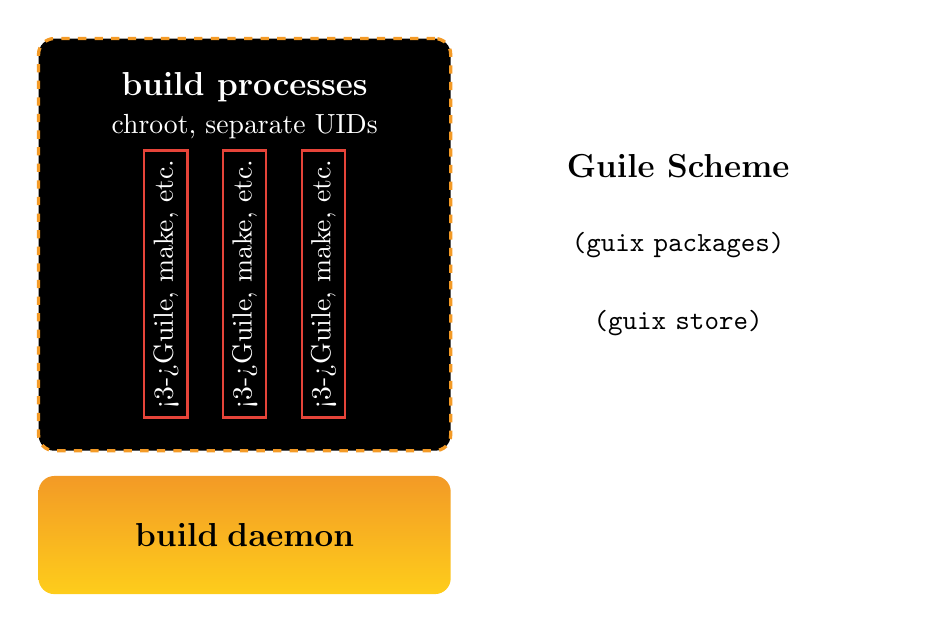
\begin{tikzpicture}[tools/.style = {
                        text width=35mm, minimum height=4cm,
                        text centered,
                        rounded corners=2mm,
                        fill=white, text=black
                      },
                      tool/.style = {
                        fill=white, text=black, text width=3cm,
                        text centered
                      },
                      daemon/.style = {
                        rectangle, text width=50mm, text centered,
                        rounded corners=2mm, minimum height=15mm,
                        top color=guixorange1,
                        bottom color=guixyellow,
                        text=black
                      },
                      builders/.style = {
                        draw=guixorange1, very thick, dashed,
                        fill=black, text=white, text width=5cm,
                        rounded corners=2mm,
                      },
                      builder/.style = {
                        draw=guixred2, thick, rectangle,
                        fill=black, text=white,
                        rotate=90
                      }]
    \matrix[row sep=3mm, column sep=1cm] {
      \node(builders)[builders, text height=5cm]{}
          node[fill=black, text=white] at (0, 2) {\large{\textbf{build processes}}}
          node[fill=black, text=white] at (0, 1.5) {chroot, separate UIDs}
          node[builder, onslide=<1-2>{black}] at (-1,-0.5) {\alert<3->{Guile}, make, etc.}
          node[builder, onslide=<1-2>{black}] at ( 0,-0.5) {\alert<3->{Guile}, make, etc.}
          node[builder, onslide=<1-2>{black}] at ( 1,-0.5) {\alert<3->{Guile}, make, etc.}; &
      \node[tools]{}
          node[fill=white, text=black] at (0, 1) {\large{\textbf{Guile Scheme}}}
          node[tool] at (0, 0) {\texttt{(guix packages)}}
          node(client)[tool] at (0, -1) {\texttt{(guix store)}};
      \\

      \node(daemon)[daemon]{\large{\textbf{build daemon}}}; &
      &
      \\
    };
  \end{tikzpicture}

  \begin{tikzpicture}[overlay]
    \path[very thick, draw=guixorange1]<2->
      (client.south) edge [out=-90, in=0, ->] node[below, sloped]{RPCs} (daemon.east);
    \path[->, very thick, draw=guixorange1]<3->
      (daemon) edge (builders);
  \end{tikzpicture}
\end{frame}

\begin{frame}[plain]
  \Huge{\#3. From packages to derivations.}
\end{frame}

\setbeamercolor*{normal text}{fg=black,bg=white}
\begin{frame}[plain]
  \begin{tikzpicture}[overlay]
    \node [at=(current page.center), inner sep=0mm]{
      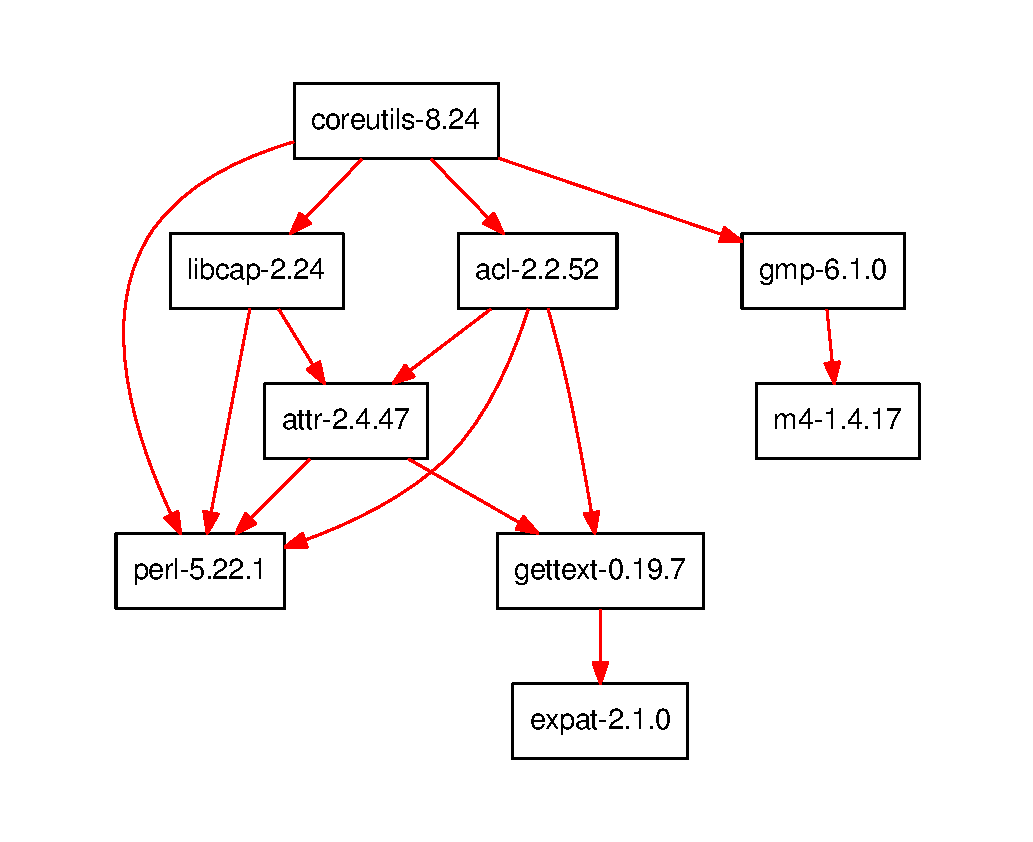
\includegraphics[width=\textwidth]{images/coreutils-graph}
    };
    \node (command) [at=(current page.south east), text=black,
        text opacity=1., anchor=south east, inner sep=3mm]{
      \texttt{guix graph --type=\textbf{package} coreutils}
    };
    \node [at=(current page.south west), anchor=south west,
           inner sep=3mm, text=black, text opacity=1]{
      \Large{\textbf{9 nodes}}
    };
    \node<2->[fill=guixorange1, text=black, text opacity=1, opacity=.7,
      rounded corners=2mm, inner sep=5mm, at=(current page.center)] {
      \textbf{\Large{Where are GCC, libc, etc.?}}
    };
  \end{tikzpicture}
\end{frame}

\begin{frame}[plain]
  \begin{tikzpicture}[overlay]
    \node [at=(current page.center), inner sep=0mm]{
      \includegraphics[width=\textwidth]{images/coreutils-emerged-graph}
    };
    \node [at=(current page.south west), anchor=south west,
      inner sep=3mm, text=black, text opacity=1]{
      \Large{\textbf{28 nodes}}
    };
    \node [at=(current page.south east), anchor=south east,
      inner sep=3mm, text=black, text opacity=1]{
      \texttt{guix graph --type=bag-emerged coreutils}
    };
    \node<2->[fill=guixorange1, text=black, text opacity=1, opacity=.7,
      rounded corners=2mm, inner sep=5mm, at=(current page.center)] {
      \textbf{\Large{What about the compiler's compiler, etc.?}}
    };
  \end{tikzpicture}
\end{frame}

\begin{frame}[plain]
  \begin{tikzpicture}[overlay]
    \node [at=(current page.center), inner sep=0mm]{
      \includegraphics[width=\textwidth]{images/coreutils-bag-graph}
    };
    \node [at=(current page.south west), anchor=south west,
      inner sep=3mm, text=black, text opacity=1]{
      \Large{\textbf{82 nodes}}
    };
    \node [at=(current page.south east), anchor=south east,
      inner sep=3mm, text=black, text opacity=1]{
      \texttt{guix graph --type=bag coreutils}
    };
  \end{tikzpicture}
\end{frame}

\begin{frame}[plain]
  \begin{tikzpicture}[overlay]
    \node [at=(current page.center), inner sep=0mm,
      inner sep=3mm, text=black, text opacity=1]{
      %\includegraphics[width=\textwidth]{images/coreutils-bag-graph}
      (too big)
    };
    \node [at=(current page.south west), anchor=south west,
      inner sep=3mm, text=black, text opacity=1]{
      \Large{\textbf{383 nodes}}
    };
    \node [at=(current page.south east), anchor=south east,
      inner sep=3mm, text=black, text opacity=1]{
      \texttt{guix graph --type=derivation coreutils}
    };
  \end{tikzpicture}
\end{frame}
\setbeamercolor*{normal text}{fg=white,bg=black}

\begin{frame}[plain, fragile]
  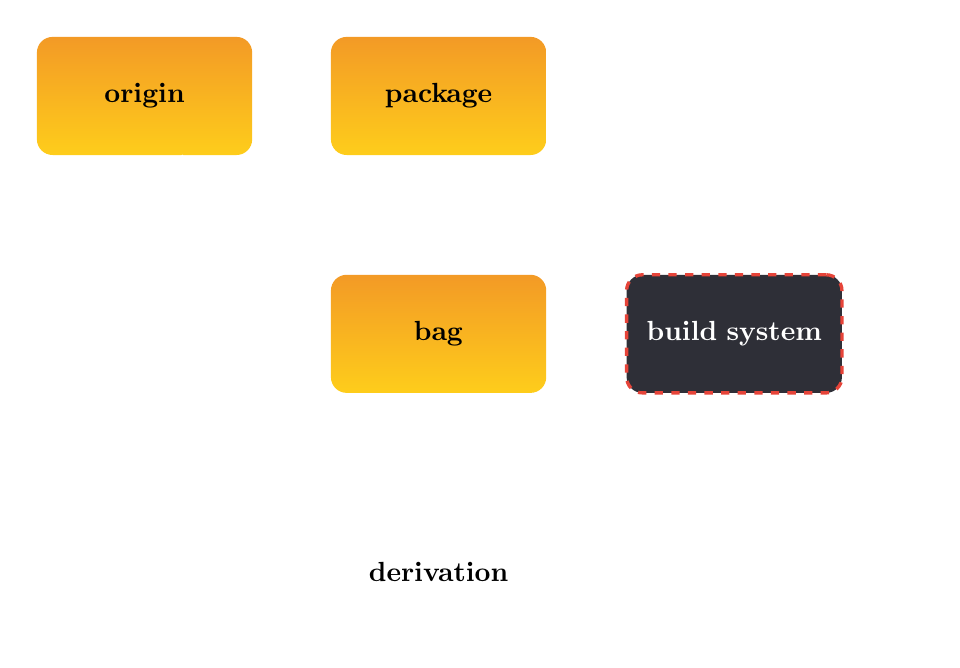
\begin{tikzpicture}[hilevel/.style = {
                        rectangle, text width=25mm, text centered,
                        rounded corners=2mm, minimum height=15mm,
                        top color=guixorange1,
                        bottom color=guixyellow,
                        text=black
                      },
                      buildsys/.style = {
                        rectangle, text width=25mm, text centered,
                        rounded corners=2mm, minimum height=15mm,
                        very thick, dashed, fill=guixdarkgrey,
                        text=white, text opacity=1, draw=guixred2
                      },
                      drv/.style = {
                        rectangle, text width=25mm, text centered,
                        rounded corners=2mm, minimum height=15mm,
                        fill=white, text=black
                      }]
    \matrix[row sep=15mm, column sep=1cm] {
      \node(package)[hilevel] {\textbf{origin}}; &
      \node(origin)[hilevel] {\textbf{package}}; &
      &
      \\

      & \node(bag) [hilevel] {\textbf{bag}}; &
      \node(buildsys) [buildsys] {\textbf{build system}}; &
      \\

      & \node(derivation) [drv] { \textbf{derivation} };
      & &
      \\
    };

    % bag/derivation are inverted!  XXX
    \path[->, very thick, draw=white, sloped] (origin) edge (bag);
    \path[->, very thick, draw=white] (bag) edge (derivation);
    \path[->, very thick, draw=white] (package) edge (derivation);
  \end{tikzpicture}
\end{frame}

\begin{frame}[plain]
  \Huge{\#4. ``Staging'': hosting build-side code.}
\end{frame}

\begin{frame}[fragile]{}
  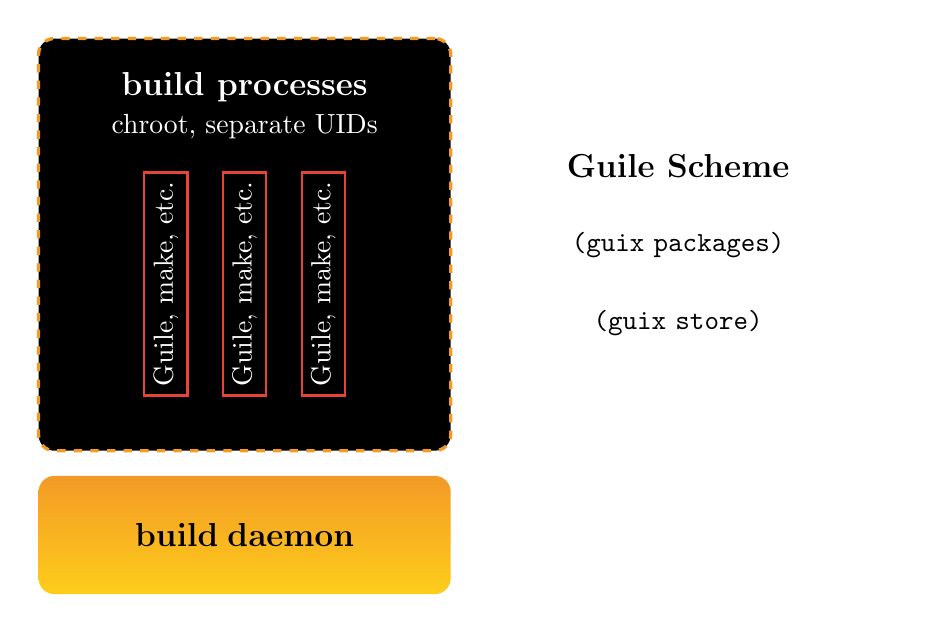
\begin{tikzpicture}[tools/.style = {
                        text width=35mm, minimum height=4cm,
                        text centered,
                        rounded corners=2mm,
                        fill=white, text=black
                      },
                      tool/.style = {
                        fill=white, text=black, text width=3cm,
                        text centered
                      },
                      daemon/.style = {
                        rectangle, text width=50mm, text centered,
                        rounded corners=2mm, minimum height=15mm,
                        top color=guixorange1,
                        bottom color=guixyellow,
                        text=black
                      },
                      builders/.style = {
                        draw=guixorange1, very thick, dashed,
                        fill=black, text=white, text width=5cm,
                        rounded corners=2mm,
                      },
                      builder/.style = {
                        draw=guixred2, thick, rectangle,
                        fill=black, text=white,
                        rotate=90
                      }]
    \matrix[row sep=3mm, column sep=1cm] {
      \node(builders)[builders, text height=5cm]{}
          node[fill=black, text=white] at (0, 2) {\large{\textbf{build processes}}}
          node[fill=black, text=white] at (0, 1.5) {chroot, separate UIDs}
          node[builder] at (-1,-0.5) {\alert{Guile}, make, etc.}
          node[builder] at ( 0,-0.5) {\alert{Guile}, make, etc.}
          node[builder] at ( 1,-0.5) {\alert{Guile}, make, etc.}; &
      \node[tools]{}
          node[fill=white, text=black] at (0, 1) {\large{\textbf{Guile Scheme}}}
          node[tool] at (0, 0) {\texttt{(guix packages)}}
          node(client)[tool] at (0, -1) {\texttt{(guix store)}};
      \\

      \node(daemon)[daemon]{\large{\textbf{build daemon}}}; &
      &
      \\
    };
  \end{tikzpicture}

  \begin{tikzpicture}[overlay]
    \path[very thick, draw=guixorange1]
      (client.south) edge [out=-90, in=0, ->] node[below, sloped]{RPCs} (daemon.east);
    \path[->, very thick, draw=guixorange1]
      (daemon) edge (builders);
  \end{tikzpicture}
\end{frame}

\begin{frame}[plain]
  \Huge{\#5. Operating system!}
\end{frame}

%%%%%%%%%%%%%%%%%%%%%%%%%%%%%%%%%%%%%%%%%%%%%%%%%%%%%%%%%%%%%%%%%%%%%%%%%%%%%%
\begin{frame}[plain]

\vfill{
  \vspace{2.5cm}
  \center{
\includegraphics[width=0.3\textwidth]{images/GuixSD}}\\[1.0cm]
  \texttt{ludo@gnu.org}\hfill{\alert{\url{http://gnu.org/software/guix/}}}
}

\end{frame}

\begin{frame}{}

  \begin{textblock}{12}(2, 8)
    \tiny{
      Copyright \copyright{} 2010, 2012--2016 Ludovic Courtès \texttt{ludo@gnu.org}.\\[3.0mm]
      GNU GuixSD logo, CC-BY-SA 4.0, \url{http://gnu.org/s/guix/graphics}

      Copyright of other images included in this document is held by
      their respective owners.
      \\[3.0mm]
      This work is licensed under the \alert{Creative Commons
        Attribution-Share Alike 3.0} License.  To view a copy of this
      license, visit
      \url{http://creativecommons.org/licenses/by-sa/3.0/} or send a
      letter to Creative Commons, 171 Second Street, Suite 300, San
      Francisco, California, 94105, USA.
      \\[2.0mm]
      At your option, you may instead copy, distribute and/or modify
      this document under the terms of the \alert{GNU Free Documentation
        License, Version 1.3 or any later version} published by the Free
      Software Foundation; with no Invariant Sections, no Front-Cover
      Texts, and no Back-Cover Texts.  A copy of the license is
      available at \url{http://www.gnu.org/licenses/gfdl.html}.
      \\[2.0mm]
      % Give a link to the 'Transparent Copy', as per Section 3 of the GFDL.
      The source of this document is available from
      \url{http://git.sv.gnu.org/cgit/guix/maintenance.git}.
    }
  \end{textblock}
\end{frame}

\end{document}

% Local Variables:
% coding: utf-8
% comment-start: "%"
% comment-end: ""
% ispell-local-dictionary: "american"
% compile-command: "rubber --pdf talk.tex"
% End:

%%  LocalWords:  Reproducibility
